%!TEX root = main.tex
\chapter{TaleBlazer Analytics}

This chapter provides a high-level overview of the three different components that make up the TaleBlazer Analytics system: the analytics server, client, and website. The TaleBlazer Analytics system is described in its entirety, including specifics about each component and how the components work together to form the core of the analytics functionality. 

\section{System Overview} 

TaleBlazer Analytics is composed of three different components that work together to gather, analyze, and present gameplay metrics for TaleBlazer games. The three components are: 
	\begin{itemize}
		\item analytics server
		\item analytics client
		\item analytics website
	\end{itemize}

The analytics server is a Node.js application that is responsible for receiving, processing, and analyzing gameplay metrics, as well as serving the analytics website. It forms the backbone of the TA system. 

The analytics client is a standalone JavaScript client which is integrated into TaleBlazer Mobile and is responsbile for the actual collection of gameplay metrics and handles all the workflow of interactions between TaleBlazer Mobile and the analytics server. 

The analytics website allows users to view and download the calculated statistics for their TaleBlazer games. The site receives its information via calls to an API (Application Programming Interface) hosted by the analytics server. The site is written in JavaScript with a focus on client-side page rendering, with light server-side templating. 

\section{Analytics Server}

This section provides an in-depth explanation of the technology and development process behind the analytics server.

\subsection{Technical Overview}

The TaleBlazer Analytics server is a Node.js web application that is responsible for collecting, proessing, and analyzing all the gameplay metrics received from TaleBlazer Mobile via the analytics client. The analytics server is built using Express, a web application framework that provides a robust library for building web services. The server follows the MVC (Model-View-Controller) development pattern for structuring the application. The server is a RESTful web service, which means that all external interactions with the server occur via REST (Representational State Transfer) APIs. \cite{site:rest} MySQL is used as the backing database for analytics data.

Strict development methodologies were adopted to ensure that the server is easily modifiable, extensible, and maintainable. To this end, the analytics server is testable and extensively documented. The server was built to be easily configurable and simple to deploy in local, testing, and production environments. Deployment in production environments is simplified through the use of Nginx as a proxy server and comprehensive logging functionality.

\subsection{Server Structure}

A crucial step in developing the analytics server was deciding on the best way to structure the server. The main goal was to reach an optimum level of component decoupling, which would allow features to be easily implemented and modified without affecting unrelated parts of the application. To this end, the Express web application framework was used to provide the high-level web-oriented functionality, such as routing and HTTP request handling. The application is split up into models, views, and controllers (MVC), which separates code according to their functionality. 

\subsubsection{Express}
Express is a minimal, non-opinionated framework that provides a framework for building web applications. It is built on top of the low-level Node.js HTTP module and provides a high-level API for handling all interactions having to do with HTTP requests. At its core, Express provides simple ways of routing URLs, parsing HTTP requests, sending HTTP responses, and defining paths for request processing via middleware. Defining what code to execute based on a request to a URL (routing) is simple using Express:

\medskip
\begin{lstlisting}[caption={[Express URL Routing Example]Example of Express' URL routing}]
// Responds to a GET request at /helloWorld with the text 'Hey!'
app.get('/helloWorld', function(res, req) {
	res.send('Hey!');
});
\end{lstlisting}

Express handles incoming requests by passing a request according to a defined path of functions, known as middleware. For the analytics server, this provided the ability to implement robust error handling and logging functionality. 

\subsubsection{Model-View Controller}

Code in the analytics server is organized according to the Model-View-Controller (MVC) pattern, which allows us to separate code into logical components based on their functionality. Models represent database objects and contain retrieval and modification methods. Controllers handle incoming requests by retrieving information for specific models and sending the information the the requestor. Views contain the logic for the user interface and request information from controllers. 

\paragraph{Models} 
Models in the analytics server correspond directly to their respective database tables and allow us to easily perform queries on the database without having to write SQL. This is accomplished via Sequelize, an object-relational mapping (ORM) library, which handles the database connection and abstracts SQL queries and relations between tables by providing a high-level JavaScript API. Sequelize also provides migration functionality, which lets us make incremental changes to the database schema. Additionally, it performs model validation prior to making any database calls for an extra level of security.

The models for TaleBlazer Server represent exactly the types of information as defined in section \ref{sec:analytics_data}, with the following exceptions and additions:

	\begin{enumerate}
		\item Custom events are represented jointly by a Custom Event and Custom Event Trigger model
		\item Games are represented by a Draft and Draft State model.
	\end{enumerate}

\subparagraph{Custom Events}
	Data about custom events is split up into two models: Custom Events and Custom Event Triggers. The Custom Events model contains information the unique ID and name of the event, as well as what game it belongs to.
	The Custom Event Trigger model represents an actual instance of a custom event i.e. the time the event occurred, the value of the custom event block, the ID of the session it occurred in, and a reference to the Custom Event model whose instance the trigger represents.

	The Custom Event model exists on its own due to the process of database normalization. This process structures database tables so as to avoid unnecessary repetition of information. As a result, normalized database tables perform at optimal speeds. In particular, the existence of the Custom Event model allows us to quickly retrieve all custom events associated with a particular game, which is necessary in the final analytics site.

\subparagraph{Games}
	In the database (and the corresponding model), a game is represented by a Draft and a Draft State. Drafts contain information consistent throughout all versions of a game, such as the user who made it and the the most recent version of the game. Draft States represent versions of a game and contain information specific to a particular game version, such as the name of the game and its description. Draft States also contain the ID of the Draft that they belong to.

% Need to differentiate this from the previous subparagraph
\paragraph{Controllers} 

Controllers for the analytics server handle, process, and respond to requests. Each controller provides the functions that get executed when a URL is requested. For example, requests to register or get information about a device will always go through the device controller. In particular, controllers can be split up into two groups: data collection and data analysis controllers.

\paragraph{Views}

The analytics server also serves the analytics site and as such is responsible for providing the HTML, JavaScript, and CSS resources required for page of the analytics site. Dynamic page content for the analytics site is largely performed by client-side JavaScript. However, a minimal amount of HTML template rendering is performed on the server. Views correspond directly to these HTML templates, which contain the markup for the page layout. The ECT JavaScript template engine powers the template rendering and allows us to split up templates into logical components, thereby making it easier to modify the pages of the analytics site.


\subsection{REST API}

All external interactions with the analytics server occur through a REST API. All API endpoints return JSON (JavaScript Object Notation) and conform to a standard response format. For consistency and standards-compliance, each endpoint enforces that the correct HTTP headers be set and responds with the correct HTTP status code for the state of the response.

The analytics server API endpoints are divided into two groups:
	\begin{itemize}
		\item the data collection API, used to collect data from TaleBlazer Mobile
		\item the data analysis API, used to provide statistics for the analytics site
	\end{itemize}


\subsubsection{What is REST?}
REST, standing for Representation State Transfer, is a style for building HTTP APIs, using the HTTP verbs (GET, POST, PUT, DELETE) as actions on resources. A resource can be thought of as a noun (e.g. the device resource). Basic CRUD (create, update, read, delete [maybe put in glossary]) operations can be performed by making a request to a resource using a particular format. For example, a GET request to \texttt{http://SITE/device/4} would return a device with id equal to 4. 

\subsubsection{API Format}

Each API endpoint responds with JSON formatted according to the JSEND format. \cite{site:jsend} Each response object has a ``status'' key, which has a value of ``success'' or ``error'' depending on the outcome of the request. Successful response include a ``data'' key, which contains data pertinent to the original request. Failure responses include a ``message'' key, containing a Javascript Error object or human-readable string describing the error. Conforming to a standard response format makes it simpler to parse responses to API requests and maintains consistency throughout the project. Listing \ref{lst:jsend} gives an example of the response body of a succesful request to the device API.

\medskip
\begin{lstlisting}[caption={[API Response Format Example]Example API format, using JSEND}, label={lst:jsend}]
{
    status : "success",
    data : {
        "device" : { "id" : 1, "model" : "iPhone 5", ...}
     }
}
\end{lstlisting}

All API endpoints require correct HTTP headers for requests. For example, the ``Content-Type'' header, which defines the format of parameters in the request body, must be set to ``application/json'' if in JSON format. Similarly, the ``Accepts'' header, which defines acceptable formats for the response, must be set to ``application/json'' in order for the response to return JSON. Again, this ensures that API requests behave consistently and correctly; inconsistent or undefined behavior often leads to bugs.

In addition to the status field in the JSON response, each endpoint also responds with the correct HTTP status codes. For example, a status code of 500 represents an internal server error. A status code of 201 represents that a resource was succesfully created. These status codes provide an additional way to check the status of an API request.

\subsubsection{Data Collection API}
\label{subsec:collection_api}

The data collection API consists of all API endpoints that are involved in the process of gathering gameplay metrics from TaleBlazer Mobile. The data collection API consists of three resources: devices, sessions, and events. With respect to the process of data collection, the following endpoints are the most important:
	\begin{itemize}
		\item Device Registration,
		\item Session Requests,
		\item Batch Event Processing
	\end{itemize}

\paragraph{Device Registration}

The device registration API provides a way to register mobile devices with the analytics server. The endpoint takes a unique TaleBlazer Analytics ID and information about the device (as in \ref{subsec:device}).If successful, the API responds with a record of the newly registered device.

\paragraph{Session Request}

The session request API allows gameplay sessions to be recorded on the analytics server. It takes the device's unique TA ID and information about the session (as in \ref{subsec:session}). If the device has not already been registered with the analytics server, then the API sends back a failure response. Otherwise, it responds with a record of the newly created session, including the unique session ID used to tie events and sessions together.

\paragraph{Batch Event Processing}

The batch event processing API is the most complex in the data collection group. The batch event API takes a list of event objects, each corresponding to the types of events previously mentioned (e.g. agent bumps or region switches) and saves each event to the database. If a single event in the list of events is invalid or an error occurs while saving an event, then the entire request fails and the API responds with a failure. This is accomplished through the use of database transactions, which provide an ``all-or-nothing'' guarantee: either everything is saved or nothing is. This is beneficial because it alerts the API user that an error has occurred and that no data was saved. Otherwise, it would be difficult to tell what was saved to the database and what wasn't. As a result, it provides consistent ``fail-fast'' behavior for the API and avoids tracking possibly problematic data.

\subsubsection{Data Analysis API}
\label{subsec:analysis_api}

The data analysis API consists of the API endpoints that calculate and provide analytics data for the analytics site. Currently, all statistics are calculated on-the-fly when requested via the API. The data analytics API consists of the following endpoints:
	\begin{itemize}
		\item Overview
		\item Games Played
		\item Gameplay Duration
		\item Agent Bumps
		\item Custom Events
		\item Raw Data
	\end{itemize}

Each API takes a start and end date representing the date range of data to analyze. Excluding the Overview API, they also take a categorization method, which categorizes the data based on one of the following:
	\begin{itemize}
		\item Date (Excluding the Agent Bumps API)
		\item Role
		\item Scenario
		\item Game Version
		\item Agent Bump (Only for the Agent Bumps API)
	\end{itemize}

\paragraph{Overview}

The Overview API provides key statistics concerning the overall performance of a game. The statistics that are calculated include the number of games initiated, the number of games completed, the average time users took to complete a game, and the lifetime number of downloads. This information is calculated purely from information on the Session model (Section \ref{subsec:session}).

\paragraph{Games Played}

The Games Played API responds with information about the total number of games played. This is further broken down into non-overlapping groups:
	\begin{itemize}
		\item the number of games initiated (but not completed)
		\item the number of games completed
	\end{itemize}

These statistics are calculated solely from information on the Session model, as in the Overview API.

\paragraph{Gameplay Duration}

The Gameplay Duration API provides statistics on the amount of time that people took to play a game. In particular, gameplay sessions are separated into buckets based on their gameplay time. Currently, sessions are bucketed into time ranges of 15 minutes, starting at 0 minutes and going up to 120 minutes. Listing \ref{lst:duration_response} demonstrates a sample response.

\medskip
\begin{lstlisting}[caption={[Gameplay Duration API Response Example]Gameplay Duration API response{,} showing the number of sessions that fell within certain ranges of gameplay time{,} categorized by the Explorer role}, label={lst:duration_response}]
{
  "status": "success",
  "data": {
    "results": [
      {
        "0-15": 3,
        "15-30": 4,
        "30-45": 0,
        "45-60": 6,
        "60-75": 3,
        "75-90": 5,
        "90-105": 1,
        "105-120": 4,
        "120+": 0,
        "role": 1,
        "entityName": "Explorer"
      }
    ]
  }
}
\end{lstlisting}

As before, all information is directly calculated from information on the Session model.

\paragraph{Agent Bumps}

The Agent Bumps API provides information about the number of times an agent was bumped, divided into unique bumps and total bumps by agent. Unique bumps are calculated by determining if a particular agent was bumped at all during a session. Further bumps then contribute to the number of total bumps. 

\paragraph{Custom Events}

Similar to the Agent Bumps API, the Custom Events API gives statistics as to how many unique and overall custom events were triggered. Unique and total events are calculated as in the Agent Bumps API. Due to the fact that custom events can have any set of values, custom events are further grouped by their particular value, in addition to the normal categorization options.

\paragraph{Raw Data}

The Raw Data API is the sole exception to the standard JSON format. Instead of JSON, the Raw Data API responds with a CSV of all the raw event data for a particular game over a given date range. The purpose of this endpoint is to allow power users to work directly with the collected data to perform further analysis.


\subsection{Development Methodology}

In addition to the goal of collecting and analyzing gameplay data, a goal of the project was to develop a maintainable server that was easily modifiable and extensible in order to allow future developers to easily add features and continue building atop the platform. To this end, a test-driven methodology of development was adopted and stringent documentation standards were employed throughout development


\subsubsection{Test-Driven Development}

The analytics server was developed according to the Test-Driven Development (TDD) methodology. This methodology emphasizes that tests for logical chunks of functionality be written first before starting development on the feature. As a result, the developer is forced to consider in-depth the behavior of the feature and the success and failure conditions. On completion of a feature, the tests are run and the feature deemed complete if all the tests pass. This results in a codebase with extensive test coverage. Furthermore, the overall test suite provides a way of verifying that changes to the codebase do not accidentally break functionality. 

For the analytics server, this methodology resulted in extensive test coverage for the API. Tests were written using the Mocha testing framework and the SuperTest HTTP assertion library. These libraries emphasize readable and self-documenting tests. For example, Listing \ref{lst:mocha_example} shows how a test is written.

\medskip
\begin{lstlisting}[caption={[Example API Test]Example Mocha test{,} testing that the Session API responds in JSON}, label={lst:mocha_example}]
	it('responds with json', function(done) {
		request
			.get('/session')
			.set('Accept', 'application/json')
			.expect('Content-Type', /json/)
			.expect(200, done);
	});
\end{lstlisting}

\subsubsection{Documentation}

Documentation for the analytics server was a continuous and simultaneous process alongside development. The overall goal was to write clear and useful documentation. The codebase was documented in two ways. First, the code was written to be as self-documenting as possible, using clear and descriptive variable names. Code linters and style formatters were employed consistently throughout the development process to enhance readability and ensure style consistency throughout the various files. Second, comments were added to pieces of code that required further explanation, detailing specific processes or ideas further. For example, the ideas behind statistic calculations were expanded on in comments.

In addition to the documentation inside the codebase, detailed step-by-step instructions were written explaining how to install and deploy the server. Documentation also included pre-built files for performing test API requests using an external utility and a file giving an overview of the database schema.

This documentation standard was also employed for the development of the analytics client and site.

\subsection{Installation and Deployment}

\subsubsection{Configuration and Installation}

To simplify future development and deployment, the server was built to be easily configurable and simple to deploy to any environment. Server configuration comes in the form of external JSON files and JavaScript modules that contain server and database configuration details. Example configuration files are provided to ease the setup process. 

Installation and deployment to any environment is similarly simple. Developers simply checkout the project from a Git repository, fill in their configuration details, and run a single command to start the server. As a result, getting started developing for the analytics server is fast and easy. 

\subsubsection{Logging}

Logging functionality was implemented into the server in order to simplify troubleshooting in production and environments. Logging is handled via Winston, an asynchronous logging library for Node.js. To ease troubleshooting, error and request logs are saved to log directory, configurable by the developer. Error logs contain stacktraces, server performance statistics, and additional error-related information.

\subsubsection{Deployment alongside TaleBlazer Server}

The TaleBlazer Analytics server was deployed on the same machines as the existing TaleBlazer server. Early testing with our partners indicated that certain networks would restrict access via HTTP to sites on ports other than port 80. As a result, it was necessary to find a way to deploy TaleBlazer server and the analytics server alongside each other and have both servers respond to requests at port 80. Nginx was deployed as a reverse proxy server to accomplish this. 

Nginx is a high-performance HTTP server which is often used as a reverse proxy or load-balancer in front of other servers. A reverse proxy server is a server which retrieves information from other servers on behalf of a client making a request. In our particular case, Nginx allows TaleBlazer server and analytics to both respond to requests on port 80. It accomplishes this by performing requests to the respective server on behalf of the original client and then serving the request. Fitting with the goals of the project, Nginx is also easily deployed and configured.

\section{TaleBlazer Analytics Client}

This section provides the technical details of how the TaleBlazer Analytics is built and how it interacts with the analytics server to collect gameplay data. 

\subsection{Technical Overview}

The TaleBlazer Analytics client is standalone JavaScript module that handles the API workflow for collecting data from TaleBlazer Mobile. TaleBlazer Mobile implements the client's public API to track gameplay events. The client is then responsbile for the storage of gameplay data and for interacting with the analytics server to save those events. 

The TaleBlazer Analytics client is designed to function in both offline and online capacities. TaleBlazer games can be played in offline situations, where internet connectivity is not available. In order to track this data, the analytics client stores all gameplay data locally until a data connection becomes available, at which point it sends the data to the server for storage.

\subsection{API Workflow}
\label{subsec:api_workflow}

The main job of the analytics client is to interact with the Data Collection API (see \ref{subsec:collection_api}) of the analytics server to track gameplay data gathered from TaleBlazer Mobile. To track data, a specific workflow has to be followed in order to ensure that data is collected from offline and online gameplay sessions. The general workflow is as follows:
	\begin{description}
		\item[First] The mobile device is registered with the analytics server.
		\item[Second] At the start of a new game, a session is requested from the analytics server.
		\item[Third] Events are periodically sent to the analytics server in batches
	\end{description}
Each step in this workflow requires that the prior steps be successfully completed. If a step fails, the client automatically retries the failed step periodically. [DIAGRAM MAYBE OF WORKFLOW?] For example, if a device is not registered with the server and a new game is started, the client will automatically attempt to register the device before requesting a session from the analytics server. In the case of TaleBlazer games played offline or in low connectivity situations, the client generates local sessions to be able to track events. The above workflow is then performed once network connectivity is regained in order to record data with the analytics server.

\subsubsection{Device Registration}

In order to determine unique events, it is necessary to register each mobile device with server. When TaleBlazer Mobile is launched, the client attempts to register the mobile device with the analytics server.
If the device is sucessfully registered or the server responds that the device has already been registered, the client stores that information locally so as to avoid further unnecessary registration requests. The information sent up to the server is that mentioned in subsection \ref{subsec:device}. 

In order to ensure that data is truly anonymous, a unique TaleBlazer Analytics specific device ID is generated from the device's ID. On iOS, this ID is an install-specific which changes if the user reinstalls the app. On Android, this could be the device's actual device ID, depending on the version of the OS. To generate a unique ID specific for our purposes, the retrieved device ID is hashed with the SHA-256 cryptographic algorithm. SHA-256 is a ``one-way'' cryptographic function - the generated text cannot be decrypted back to the original text. This unique generated string is used by the analytics server to uniquely identify devices. 

\subsubsection{Session Request}
\label{subsubsec:session_request}

In order to track gameplay sessions, a session has to be requested from the server at the start of a new game, with the information as defined in subsection \ref{subsec:session}. On a successful request, the server responds with a unique session ID, which the client stores locally. The session ID is used to tag events to identify them as having taken place during a particular session. Sessions can only be requested once the device has been registered, as each session is tied to the device being used.

The TaleBlazer Analytics client also has to work in an offline capacity, ensuring that events are tracked and correctly recorded with the analytics server when network connectivity is reestablished. To this end, all sessions start off as ``local sessions'', each with a session ID unique to the device. Once the network becomes available, a ``network session'' is requested for each local session stored on the device. Local sessions are then converted to network sessions and any events tagged with the corresponding local session ID are updated to use the new network session ID. 

\subsubsection{Event Tracking}
Once a session has been succesfully established, events can be tracked and recorded with the server. Each event is tagged with the session ID it occurred in and the time the event took place, as well event-specific information (see \ref{sec:analytics_data}). Events are added to a queue and sent up periodically to the server in batches of configurable size. This minimizes the amount of network requests performed and the data sent, as each request includes overhead from HTTP headers. 

Events are persisted locally in order to persist through application and device restarts, as well as to ensure that data is not lost in the face of spotty network connectivity. This allows event data from offline events to be kept and automatically sent to the server when network connectivity becomes available.

\section{TaleBlazer Analytics Site}

The sections details the structure of the analytics site and its features. It also provides examples of the user interface. 

\subsection{Technical Overview}

The TaleBlazer Analytics site allows users to view and download analytics data for their games. The front-end layout is accomplished using Bootstrap, a styling framework that provides a set of pre-styled elements, grid layout system, and extensible CSS classes. Extensive JavaScript is used to provide the behavior of the site, including the dynamic generation of UI elements, such as the tables for analytics data. 

The site is built with a focus on client-side page rendering. All relevant analytics data is retrieved via AJAX calls to the Data Analysis API of the analytics server (see \ref{subsec:collection_api}). A minimal amount of server-side HTML templating is performed to provide information such as when the game was first created and a list of its custom events, for filtering and navigation purposes. The site is also responsive: mobile and tablet devices can easily view information with a UI (user interface) suited to their device. Users can also download the raw set of data from which all analytics are calculated.

\subsection{Analytics Pages}

Analytics pages are the pages of the site that provide the different types of analytics data for each game. The analytics pages of the site correspond directly to each API in the Data Analysis API group (see \ref{subsec:analysis_api}). In particular, these pages are the:
	\begin{itemize}
		\item Games Played Page
		\item Gameplay Duration Page
		\item Agent Bumps Page
		\item Custom Events Pages
	\end{itemize}
All analytics pages share the same page loading behavior and common user interface elements. A typical analytics pages looks like Figure \ref{fig:games_played}, which shows the user interface for the Games Played page.

\begin{figure}[H]
	\center{
			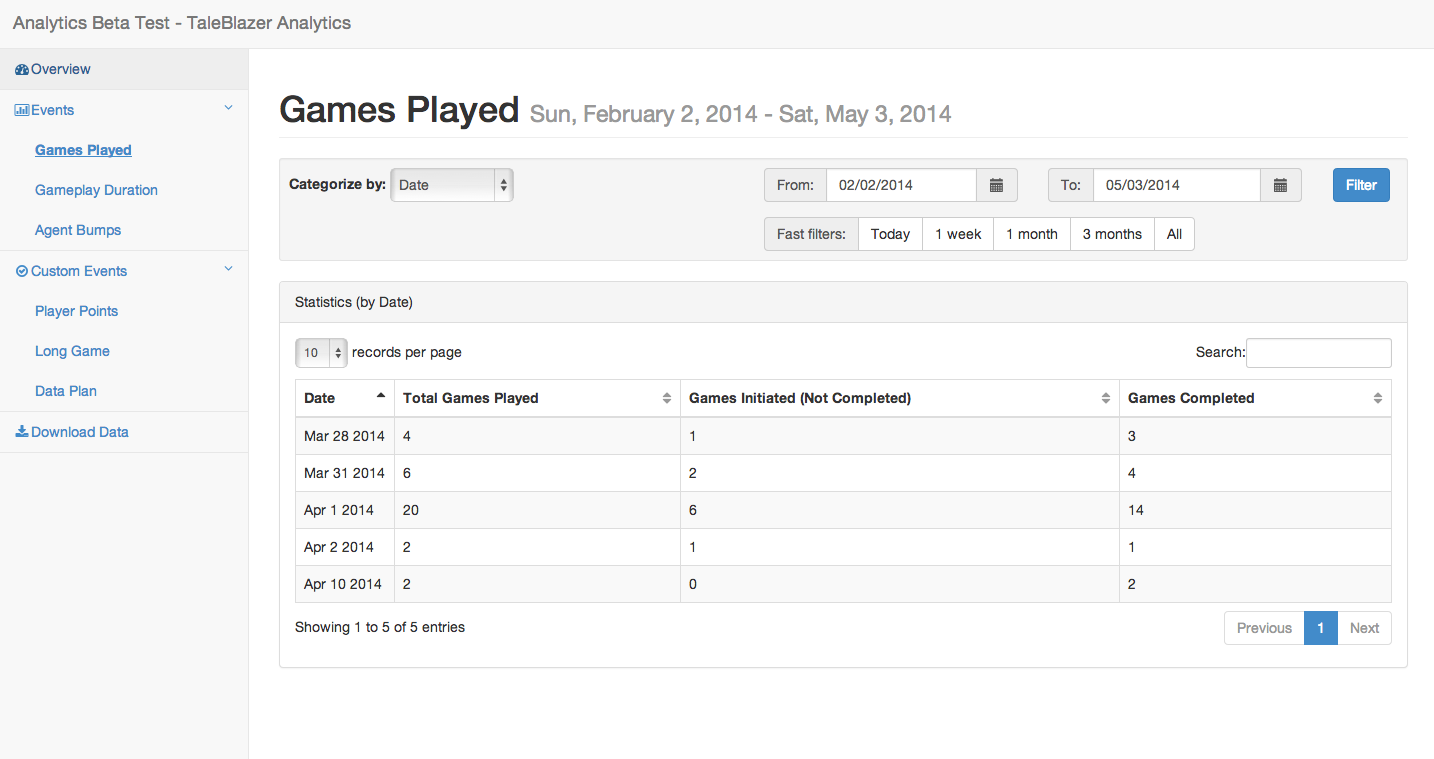
\includegraphics[width=\textwidth]
				{figures/games_played_page.png}
			}
	\caption[Analytics Site: ``Games Played'' UI]{\label{fig:games_played} Games Played Page}
\end{figure}

\subsubsection{Page Rendering and Loading}

The pages of the site all correspond directly to each API in the Data Analysis API group (see \ref{subsec:analysis_api}). For example, the Agent Bumps Page gets it HTML and analytics information from the Agent Bumps API.

HTML requests to each API return a rendered HTML page with no embedded analytics data. On the server, the page is rendered by modularly composing a set of ECT templates. This results in a modular site and accomplishes maximum code reuse. The amount of server-side templating is minimal in order to ensure that the page is rendered and served to the client as fast as possible for short page load times.

When the page is fully loaded, an AJAX (Asynchronous JavaScript and XML) call is made to the same API, which responds with the correspondng analytics data. The user interface of each page is then updated to reflect the new data. 

The combination of fast page loads and AJAX calls for data ensure that the user is not stuck looking at a loading page while the analytics data is being calculated. It also eliminates page loads when filtering and categorization options are changed and new data is requested - the page's existing UI elements are simply updated when new data is received.

\subsubsection{User Interface Elements}

All analytics pages share common user interface elements, which not only maintain consistency throughout the site, but allow maximum reuse of code. This is a result of the modular construction of each page, as previously mentioned. The common user interface elements are the site navigation menu, the filter and categorization menu, and the data table. 

\paragraph{Site Navigation Menu}

The Site Navigation Menu is a collapsible menu with links to all pages containing analytics information for a particular game. Notably, it includes a dynamic list of the custom events belonging to the game in question. Figure \ref{fig:nav_menu} shows the user interface for the menu.

\begin{figure}[htb]
	\center{
			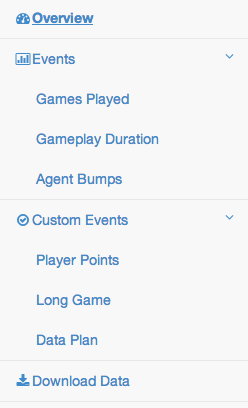
\includegraphics[scale=0.5]
				{figures/nav_menu.png}
			}
	\caption[Analytics Site: Side Navigation Menu]{\label{fig:nav_menu} Side Navigation Menu}
\end{figure}

\paragraph{Filter Menu}

The Filter Menu provides all the options for filtering and categorizing analytics data for all analytics pages. Users can choose from a pre-defined list of categories to categorize their data by. They can also manually define the date range of data they would like to look at. Additionally, they can choose from a set of pre-defined date ranges, including the option to view all data for the lifetime of the game. The list of categories can be modified or the option completely disabled on a page-by-page basis, as it is on the Overview Dashboard (Figure \ref{fig:overview_dashboard}). Figure \ref{fig:filter_menu} shows an example of the filter menu. 

\begin{figure}[hbt]
	\center{
			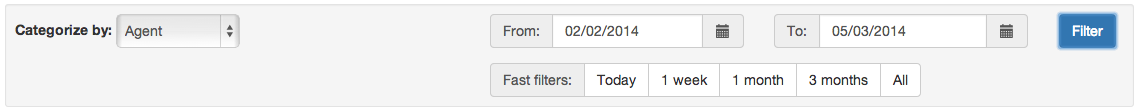
\includegraphics[width=\textwidth]
				{figures/filter_menu.png}
			}
	\caption[Analytics Site: Filter Menu]{\label{fig:filter_menu} Filter Menu, with the categorization option enabled}
\end{figure}

\paragraph{Data Table}

Each analytics page displays its analytics data in the form of a data table. This data table is implemented using the DataTable JavaScript library. Analytics data tables are column-sortable and searchable across the entire set of results. Data tables paginate automatically based on the number of results. The user can optionally choose the number of results to view per data table page. Figure \ref{fig:data_table} shows what the data table for Agent Bump data, categorized by Agent looks like. 

\begin{figure}[hbt]
	\center{
			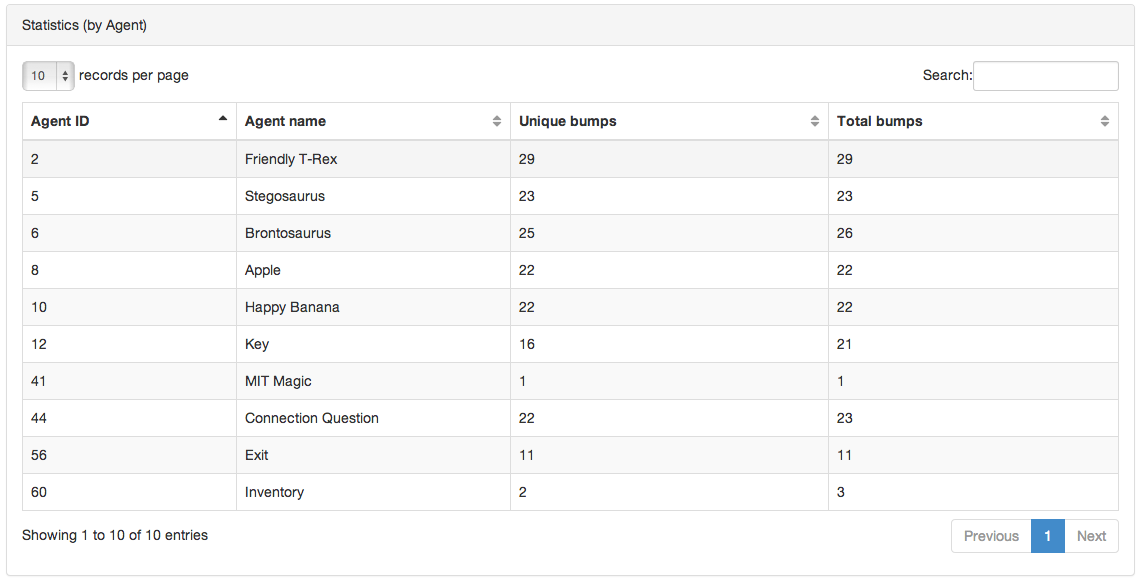
\includegraphics[width=\textwidth]
				{figures/data_table.png}
			}
	\caption[Analytics Site: Agent Bumps Data Table]{\label{fig:data_table} Data table for the Agent Bumps page, categorized by Agents}
\end{figure}

\subsubsection{Overview Dashboard}

The Overview Dashboard is a unique analytics page as it does not include a categorization option or a data table. Instead, the Overview Dashboard provides a concise set of statistics detailing the performance of the game in the form of a grid. As before, users can choose the date range of data to get statistics for. Figure \ref{fig:overview_dashboard} shows the UI for the Overview Dashboard.

\begin{figure}[hbt]
	\center{
			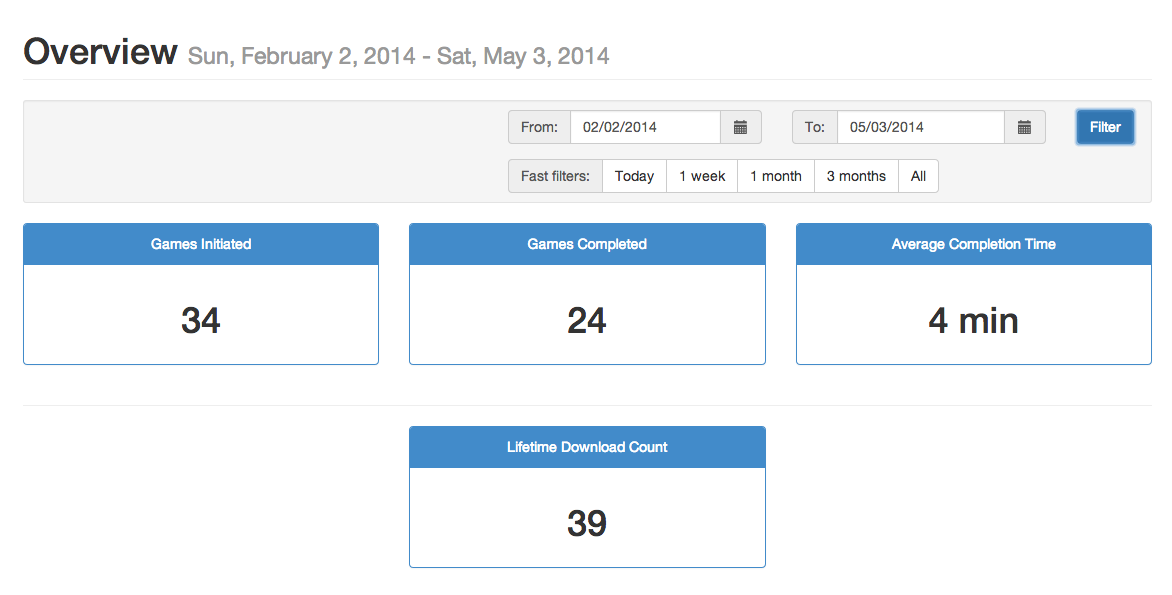
\includegraphics[width=\textwidth]
				{figures/overview_dashboard.png}
			}
	\caption[Analytics Site: Overview Dashboard]{\label{fig:overview_dashboard} Overview Dashboard}
\end{figure}


\subsection{Data Download}

The analytics site also allows users to perform their own data analysis on the collected data. Users can download a CSV (Comma-Separated Value) file containing the set of all events that occurred over a particular time period. In particular, this file contains all Agent Bump, Region Switch, and Custom Events that occurred, as well as information about the session that they occurred in and the version of the game that was played. 

This functionality allows users to not only perform data analysis on the events of a particular game, but also gives them the ability to view user behavior across separate games using the unique TaleBlazer Analytics device ID. 
















	




















